%% cycle4_ar_tr.tex
%
%  Spitzer Space Telescope Cycle-4 Proposal Template
%
%  Use this template for Archival Research or
%  Theoretical Research proposals.  No style file is required.
%
%  Version 1.0    16 October 2006
%
%%%  For Spitzer proposal preparation resources please visit 
%    the proposal kit web page: 
%
%%%  http://ssc.spitzer.caltech.edu/propkit/ 
%
%  **In particular, please read the Cycle-4 Call for Proposals (CP).
%  **It is the definitive document that describes the requirements
%  **necessary for your proposal.
%
%    Please address all questions regarding the proposal 
%    and observation to the Helpdesk at 
%
%%%  help@spitzer.caltech.edu
%
%
%
%%%%%%%%%%%%%%%%%%%%%%%%%%%%%%%%%%%%%%%%%%%%%%%%%%%%%%%%%%%%%%%%%%%%%%%%
%
%  The template begins here.  The font must be 12 point and the margins
%  must be at least 1-inch on all sides. 
%  Don't override this.  
%
% If you compile this and find that the text is "mushed up against
% the top of the page", the default paper size for your installation 
% of latex is A4.  In order to override this, do:
% > latex texfile # where the manuscript is in a file named texfile.tex
% > dvips -Ppdf -t letter -o texfile.ps texfile
% finally, to get nice (non-blurry, searchable) pdf do:
% > ps2pdf13 texfile.ps  texfile.pdf
% if you do not have ps2pdf13, please ask your sysadmin to install it.


\documentclass[letterpaper,12pt]{article}
\usepackage{epsfig,colortbl}
\textwidth=6.5in
\textheight=9.5in
\topmargin=-0.75in
\oddsidemargin=0.0in
\evensidemargin=0.0in
\pagestyle{myheadings}
\parindent=0in
\usepackage{subfigure}

% Please update the following line with the title of your proposal
% and your Author name (with "et al." if more than two authors).

\markright{Mapping $\mathrm{H_2}$ in SINGS Galaxies, G.\ Brunner et al.}
\pagenumbering{arabic}

\begin{document}

\section{Scientific Justification}

\subsection{Mapping Molecular Hydrogen Excitation and Mass in SINGS Galaxies}

\indent Galactic evolution is inherently correlated with molecular gas within a galaxy.  In the Milky Way Galaxy, we observe molecular gas in dense molecular clouds.  The collapse of these molecular clouds triggers a burst of star formation.  In other galaxies, we observe molecular gas trigger star formation in spiral arms via the passage of a spiral density wave (Vogel et al. 1988), within nuclear regions of galaxies (Young and Devereux 1991), and at the ends of bars in barred spiral galaxies (Sheth et al. 2000).  Thus, molecular gas serves as the fuel for star formation and is fundamentally connected with galaxy evolution.\\

%These observations provide constraints on the energy injection processes (i.e. radiative heating, shocks, turbulence) that heat the molecular gas phases as a function of position in a galaxy.  Thus, molecular gas in fundamentally connected with the evolution of a galaxy.\\

%Thus, molecular gas serves as the fuel for star formation and is fundamentally connected with galaxy evolution.\\

% through a variety of processes.

Prior to the Infrared Space Observatory (ISO) and the Spitzer Space Telescope (Spitzer), much of our knowledge of the conditions of the molecular gas in galaxies came from studies of CO emission and near-infrared $\mathrm{H_2}$ line emission.  CO rotational line emission directly traces the mass of the coldest (T = 5 - 100 K) $\mathrm{H_2}$ and near-infrared  $\mathrm{H_2}$ emission traces the hot (T  $\geq$ 1000 K) $\mathrm{H_2}$.  This left the warm (T = 100 - 1000 K) molecular gas unexplored.  With Spitzer, the warm (T = 100 - 1000 K) molecular gas is observed through the pure rotational levels of $\mathrm{H_2}$ with lower $J$ $\mathrm{H_2}$ lines tracing the 100 - 300 K $\mathrm{H_2}$ and higher $J$ lines tracing the 300 - 1000 K $\mathrm{H_2}$.  The $\mathrm{H_2}$(0-0)S(0) (28.2 $\mu$m) and $\mathrm{H_2}$(0-0)S(1) (17.0 $\mu$m) lines can both be observed with the Spitzer IRS long-low (LL) modules (14 - 38 $\mu$m, with LL1 covering 14 - 21 $\mu$m and LL2 covering 21 - 38 $\mu$m)(see figure 1); these lines trace the warm (T = 100 - 300 K) molecular gas.\\

The $Spitzer$ $Infrared$ $Nearby$ $Galaxies$ $Survey$ (SINGS) legacy program has surveyed 75 nearby galaxies (Kennicutt et al. 2003).  These galaxies range in Hubble type, luminosity, star formation, and nuclear activity.  The SINGS legacy has used the Spitzer IRS LL (LL1 and LL2)  module in spectral mapping mode to map radial strips across 65 galaxies within their sample.  The radial strips cover a range of dynamically distinct regions within galaxies (i.e. nuclei, spiral arms, HII regions, etc.).  The strips are roughly 50 x 600 arcsec in area and give us spatially resolved spectra (at a resolution of $\sim$ 5 arcsec) across the galaxies (figure 2).  {\bf These strips contain a wealth of data on the spatial distribution of molecular hydrogen yet to be studied.}\\

%In addition to observing $\mathrm{H_2}$ S(0) and $\mathrm{H_2}$ S(1) in the LL strips, there are a atomic features ([NeIII] (15.55 $\mu$m), [SIII](18.71 $\mu$m), [FeII](25.98 $\mu$m), [OIV](25.89 $\mu$m), [SIII](33.48 $\mu$m), and [SiII](34.82 $\mu$m) and broad PAH complexes  at 16.4 $\mu$m and 17.0 $\mu$m (Smith et al. 2004).\\

%While the SINGS team is currently studying the $\mathrm{H_2}$ lines (Roussel et al. 2007, in preparation), {\bf they have only done so for the nuclear regions} of the SINGS sample.  Their study of the $\mathrm{H_2}$ uses aperture averaged spectra over the nuclei  of the 65 galaxies to determine the excitation-temperature, mass, and ortho-to-para ratio (OPR) of $\mathrm{H_2}$ within the galaxies.  Their study {\bf does not} explore $\mathrm{H_2}$ outside of the nuclei of the galaxies and they {\bf do not} take advantage of the spatial resolution of the spectra across the galaxy.\\

{\bf We propose to take advantage of the spectacular SINGS IRS LL coverage across both the nuclear regions and disks in order to understand the spatial distribution of the warm (T = 100 - 300 K) $\mathrm{H_2}$ across a sample of 18 galaxies that have been observed by both SINGS and the  Berkeley-Illinois-Maryland-Array Survey of Nearby Galaxies (BIMA SONG) (Regan et al. 2001, Helfer et al. 2003)}.  The 18 galaxies (listed in table 1) have been studied as part of BIMA SONG  for which we have CO (J = 1 - 0) maps for each galaxy.  CO (J = 1 - 0) emission traces the cold (T = 5 - 10 K) $\mathrm{H_2}$ and the maps allow us to understand the spatial distribution of the cold $\mathrm{H_2}$ mass.  We will use the SINGS LL data cubes to map the $\mathrm{H_2}$ S(0) and $\mathrm{H_2}$ S(1) lines across the galaxies.  From these lines we will model the warm $\mathrm{H_2}$ mass, excitation-temperature, and UV radiation field across the galaxies (Kaufman et al. 2006).  We will correlate the cold $\mathrm{H_2}$ (traced by CO emission), warm $\mathrm{H_2}$ (traced by the $\mathrm{H_2}$(0-0)S(0) and $\mathrm{H_2}$(0-0)S(1) emission), and hot (traced by $\mathrm{H_2}$(2-1)S(1)(2.248 $\mu$m) and $\mathrm{H_2}$(1-0)S(1)(2.121 $\mu$m emission)  in order to understand the relationship between different $\mathrm{H_2}$ mass phases.  Additionally, we would like to understand the $\mathrm{H_2}$ excitation mechanisms by comparing the $\mathrm{H_2}$ distribution to UV and optical imagery (U, B, V, R, and $\mathrm{H_\alpha}$) and the mid-infrared spectral diagnostics ([OIV](25.89 $\mu$m) as a shock diagnostic and the electron density determined by [SIII](33.48 $\mu$m)/[SIII](18.71 $\mu$m)). The latter two are also mapped from the SINGS LL data cubes.\\

%and have CO (J = 1 - 0) maps publicly available on the NASA extragalactic database (NED).  

We have used IRS spectral mapping data acquired though GO - 20138 (PI: K. Sheth) of M51a (the Whirlpool galaxy, NGC 5194) as a test case for our study (Brunner et al., submitted).  In working with M51a, {\bf we have developed unique software that takes IRS SL and LL data cubes and creates extinction corrected line flux maps}.  Our software processes IRS low resolution data cubes and then runs PAHFIT (Smith et al. 2007) through individual spectra in order to decompose mid-infrared spectra across the data cubes.  In doing this, the line flux of every spectral feature at every spatial position in our data cubes is measured and then reconstructed into a map. {\bf These maps are powerful tools for understanding the spatial variation of $\mathrm{H_2}$ and other mid-infrared spectral lines.}\\

For M51a, we had both SL and LL coverage of an overlapping strip across M51a.  We have used our software to map $\mathrm{H_2}$ S(0) and $\mathrm{H_2}$ S(1) emission across the galaxy.  Figure 3 shows the maps of the $\mathrm{H_2}$ S(0) and $\mathrm{H_2}$ S(1) emission across M51a.  We have used these lines to model the excitation-temperature and mass distribution of the warm $\mathrm{H_2}$ across M51a.  In figure 4, we show the warm mass distribution compared to the warm $\mathrm{H_2}$ excitation-temperature distribution.  We find that the $\mathrm{H_2}$ is warmest within the center of the galaxy and is coolest in the spiral arms (which contain the bulk of the $\mathrm{H_2}$ mass).  We also compared the cold $\mathrm{H_2}$ to the warm $\mathrm{H_2}$.  In the inner spiral arms, we see offsets in the location of the peak emission within the spiral arms.  Why is this?  Do we see this in other galaxies? \\

%Additionally, we are able to map $\mathrm{H_2}$ excitation-temperature and mass in spiral arms out to 7 kpc from the nucleus of the galaxy.  The SINGS LL strips cover greater distances allowing us to understand how excitation-temperature and $\mathrm{H_2}$ mass vary as a function of galactocentric radius for 18 galaxies.\\

%We have also modeled the ortho-to-para ratio (OPR) across M51a.  From our study we found that the lower pure rotational levels ($\mathrm{H_2}$ S(0), $\mathrm{H_2}$ S(1), $\mathrm{H_2}$ S(2), and $\mathrm{H_2}$ S(3)) exhibit an OPR of 3 (or very close to) in the nuclear and spiral arm regions.  Under the assumption that the OPR is 3 across the galaxies, we can map the warm $\mathrm{H_2}$ excitation-temperature and $\mathrm{H_2}$ mass across the 18 galaxies that we would like to study.\\

For the 18 galaxies observed by both SINGS and SONG (table 1) we will address the following:\\

{\bf 1. How does the warm (T = 100 - 300 K) $\mathrm{H_2}$ excitation-temperature and mass vary across dynamically distinct regions within galaxies?}  The majority of the $\mathrm{H_2}$ mass radiates in the lower energy level $\mathrm{H_2}$ lines.  In mapping the $\mathrm{H_2}$ S(0) and $\mathrm{H_2}$ S(1) lines across the LL strips we can model the $\mathrm{H_2}$ excitation-temperature and mass distributions across the galaxies (Rigopoulou et al. 2002, Higdon et al. 2006). In addition to modeling the $\mathrm{H_2}$ excitation and mass across the galaxies, we will use $\mathrm{H_2}$ S(0) and $\mathrm{H_2}$ S(1) line ratios to model the radiation field across the galaxies (Kaufman et al. 2006).  This will allow us to undertand how the $\mathrm{H_2}$ excitation and mass vary between the nucleus, spiral arms, inter-arm regions, and dust lanes within the galaxies. These observations provide constraints on the energy injection processes (i.e. radiative heating, shocks, turbulence) that heat the molecular phases as a function of position in a galaxy.\\

{\bf 2.  How do the cold and warm $\mathrm{H_2}$ correlate across dynamically distinct regions in galaxies?  Are there offsets in the location of the warm and cold $\mathrm{H_2}$?  If so, why?}  CO (J = 1 - 0) emission traces the cold (T = 5 - 10 K) $\mathrm{H_2}$.  The combination of CO data and the $\mathrm{H_2}$ lines for every galaxy will allow us to correlate the different molecular gas phases.  Is the warm molecular gas strongly associated with the surface layers of giant molecular clouds or an inter-arm component that is bright in $\mathrm{H_2}$ but devoid of CO?  We find that in M51a, the warm and cold $\mathrm{H_2}$ are offset in different regions.  Do we observe offsets in the location of warm and cold $\mathrm{H_2}$ in other galaxies?  Offsets in the location of the cold and warm $\mathrm{H_2}$ are most likely due to the heating sources (such as massive star formation) which we can examine from U, B, V, R, and $\mathrm{H_{\alpha}}$ data.  The U, B, V, R and $\mathrm{H_{\alpha}}$ imagery provide a means to identify actively star forming regions within spiral galaxies and determine the age, metallicity, and star formation rate of actively star forming galaxies (Talbot et al. 1979, Jensen et al. 1981, Calzetti et al. 2005).\\

{\bf 3. How do the warm and hot $\mathrm{H_2}$ phases correlate across each galaxy?}  We will be applying for time on the UKIRT in order to acquire narrow band images of the $\mathrm{H_2}$(2-1)S(1) and $\mathrm{H_2}$(1-0)S(1) lines across each galaxy (and NGC 5194).  This combination of spatially resolved $\mathrm{H_2}$ emission across each galaxy will allow us to understand the behavior of the varying molecular gas phases in galaxies.\\

%We will compare optical and UV emission to $\mathrm{H_2}$ mass in order to understand the origin of offsets in the location of cold and warm $\mathrm{H_2}$.\\

%Offsets in the location of the cold and warm $\mathrm{H_2}$ are most likely due to the potential heating sources (such as massive star formation or embedded star formation) which we can readily examine from $\mathrm{H_{\alpha}}$ emission and MIPS 24 $\mu$m emission (maps of both are readily available ancillary data).\\ 

{\bf 4.  How do the warm and cold $\mathrm{H_2}$ mass correlate with the mid-infrared spectral diagnostics?}  The [OIV](25.89 $\mu$m) line has been observed to arise from shocks, the stellar winds of Wolf-Rayet stars, high-mass star photoionization, and active galactic nuclei (Schaerer and Stasinska 1999, Lutz et al. 1998, Smtih et al. 2004).  With our software, we are able to de-blend the [FeII](25.98 $\mu$m) and [OIV](25.89 $\mu$m) lines.  This allows us to discern regions where shocks are exciting the ISM.  If we observe [OIV](25.89 $\mu$m) emission coinciding with $\mathrm{H_2}$, this would imply that the $\mathrm{H_2}$ is excited by shocks.  Additionally, the ratio of the [SIII](33.48 $\mu$m) and [SIII](18.71 $\mu$m) lines provide a determination of the electron density in HII regions.  Comparison to the $\mathrm{H_2}$ data will allow us to determing the location of cold and warm $\mathrm{H_2}$ to the hot ionized gas (and thus the sites of current star formation) in HII regions.  

%This will allow us to understand the relationship of the hot ionized gas and and the warm and cold molecular gas within the spiral arms of galaxies.  We will use our ability to spatially resolve the mid-infrared emission features to discern the excitation mechanism of warm $\mathrm{H_2}$ in dynamically different regions of the galaxies.\\

\subsection{Utilizing the SINGS Legacy}

Our study will extend the SINGS mission and utilize the data products of the SINGS program.  The SINGS legacy has delivered maps of bright infrared emission features from the LL radial strips as part of their data products.  They create emission line maps within the CUBISM software and are only able to produce maps of emission features that are very bright across the entire galaxy.  The line maps that they have delivered are of [NeIII](15.5 $\mu$m) and [SiII](34.8 $\mu$m) line emission (Kennicutt et al. 2003).  {\bf Our software produces maps of every emission feature in the LL data cubes, even the extremely faint (such as $\mathrm{H_2}$ S(0)) or blended lines (such as [OIV](25.89 $\mu$m) and $\mathrm{H_2}$ S(1)) (see figure 3).}\\ 

To date, the SINGS legacy has not studied the spatially resolved spectra across the SL or LL data cubes.  Their studies of atomic features (Dale et al. 2006), PAHs (Smith et al. 2007), and $\mathrm{H_2}$ (Roussel et al., in press) have used aperture averaged spectra over the nuclear regions (and extranuclear HII regions in the case of Dale et al. 2006) of their galaxies. Our software, maps, and analysis of the spatially resolved $\mathrm{H_2}$ are unique and will supplement the SINGS legacy.

%\subsection{Utilizing the SINGS Legacy}

%Our study extends the SINGS mission and augments an already strong legacy program.  The SINGS legacy has delivered maps of bright infrared emission features from the LL radial strips as part of their data products.  They create emission line maps within the CUBISM software and are only able to produce maps of emission features that are very bright across the entire galaxy.  The line maps that they have delivered are of [NeIII](15.5 $\mu$m) and [SiII](34.8 $\mu$m) line emission (Kennicutt et al. 2003).  {\bf Our software produces maps of every emission feature in the LL data cubes, even the extremely faint (such as $\mathrm{H_2}$ S(0)) or blended lines (such as [OIV](25.89 $\mu$m) and $\mathrm{H_2}$ S(1)) (see figure 3).}\\ 

%To date, the SINGS legacy {\bf has not} studied the spatially resolved spectra across the SL or LL data cubes.  Their studies of atomic features (Dale et al. 2006), PAHs (Smith et al. 2007), and $\mathrm{H_2}$ (Roussel et al., in press) have used aperture averaged spectra over the nuclear regions (and extranuclear HII regions in the case of Dale et al. 2006) of their galaxies. Our software, maps, and analysis of the spatially resolved $\mathrm{H_2}$ are unique and will supplement the SINGS legacy.

%The comparison of $\mathrm{H_2}$ emission to other mid-infrared spectral diagnostics will allow us to understand the conditions of the ISM across galaxies and the processes that excite the ISM.  In figure 3, we present maps of $\mathrm{H_2}$ S(0), $\mathrm{H_2}$ S(1), [OIV](25.89 $\mu$m), [SIII](33.48 $\mu$m), and [SIII](18.71 $\mu$m) from M51a.\\
\clearpage

\section{Technical Plan}

%{\bf Data Reduction:} We will construct data cubes from the IRS observations using CUBISM (citation).  Both the PI (Brunner) and Co-I (Sheth) are experts with the CUBISM software.  The PI will be responsible for producing data cubes of the galaxies.  CO maps from the BIMA survey are already reduced and they are science ready.\\

The SINGS legacy has provided IRS low resolution data cubes for 65 galaxies.  As of data release 4 (DR4), there are 16 galaxies observed by SONG that have publicly available SINGS low resolution data cubes.  Two more SONG galaxies will have data cubes available via data release 5 (DR5).  The 18 galaxies that we will study are listed in table 1.\\

Data cubes for individual SINGS galaxies are publically available.  They can be found at:\\
 http://irsa.ipac.caltech.edu/data/SPITZER/SINGS/galaxies/.\\  
 
We will also construct CUBISM cube projects (not publicly available) for each of the 18 galaxies that we will be studying. CUBISM is the data reduction software for IRS spectral cubes.  Both Brunner and Sheth are experts with the CUBISM software.\\

{\bf Data Analysis:}  $\mathrm{H_2}$ maps, atomic line maps, and PAH feature maps will be created using the software developed by the PI and Co-Is while working on M51a.  Our software has the ability to create maps of spectral features that are extremely faint and/or are blended with other spectral features.  This allows the recovery of faint $\mathrm{H_2}$ S(0) emission and the $\mathrm{H_2}$ S(1) line (blended with the  PAH 17.0 $\mu$m complex).  Our software takes both SL and LL data cubes in FITS format, processes them, and then runs PAHFIT through the cubes (Smith et al. 2007).  PAHFIT is a mid-infrared spectral fitting routine that decomposes spectra into individual components and measures the integrated line flux of features. In running our software through a data cube, we save the flux measurement for every line from 14 - 38 $\mu$m at every spatial position, and in doing so, we create maps of every feature observed in the LL data cubes.  This is a very powerful tool for understanding the spatial variation of mid-infrared spectral features, especially the $\mathrm{H_2}$ lines.  Figure 3 displays maps of the $\mathrm{H_2}$ S(0), $\mathrm{H_2}$ S(1), [OIV](25.89 $\mu$m), [SIII](18.71 $\mu$m), and [SIII](33.82 $\mu$m) emission across a strip of M51a that has been spectrally mapped with the Spitzer IRS LL modules.  The $\mathrm{H_2}$ S(1) line and the [OIV](25.89 $\mu$m) lines are blended with spectral features (the 17.0 $\mu$m PAH complex and [FeII]{25.98 $\mu$m)), respectively) but our software is able to map the emission across the entire IRS LL strip.\\

We will use maps of the $\mathrm{H_2}$ S(0) and $\mathrm{H_2}$ S(1) emission to model the warm (T = 100 - 300 K) $\mathrm{H_2}$ excitation-temperature and mass across the SINGS LL strips.  The $\mathrm{H_2}$ S(0) and $\mathrm{H_2}$ S(0) lines place constraints in the $\mathrm{H_2}$ excitation and mass within a galaxy.  Additionally, ratios of the $\mathrm{H_2}$ S(0) and $\mathrm{H_2}$ S(1) lines probe the radiation field of dense PDRs and molecular clouds in star forming regions.  Brunner and Wolfire will lead the $\mathrm{H_2}$ modeling effort.\\

We will compare the warm $\mathrm{H_2}$ mass distribution to the cold (T = 5 - 10 K) $\mathrm{H_2}$ mass distribution traced by CO emission.  We will use the MIRIAD package to analyze the CO data and we will use WIP to compare the spatial distribution of $\mathrm{H_2}$, CO, and the mid-infrared spectral diagnostics. Brunner will lead the data analysis though it should be mentioned that Brunner, Sheth, Wolfire, and Vogel all have extensive experience with MIRIAD and WIP.  Sheth and Vogel were both integral members of the BIMA collaboration and have tremendous insight into the CO data and results.  Interpretation of the $\mathrm{H_2}$ results and the comparisons of the $\mathrm{H_2}$ to CO will be shared by Brunner, Sheth, and Vogel.\\

We will also be proposing to map the $\mathrm{H_2}$(2-1)S(1) and $\mathrm{H_2}$(1-0)S(1) lines with UKIRT for each galaxy.  Brunner, Dufour, and Sheth will be responsible for the near infrared $\mathrm{H_2}$ emission observations.\\

 Comparison of the $\mathrm{H_2}$ to the U, B, V, R, and $\mathrm{H_\alpha}$ imagery and mid-infrared spectral diagnostics will be shared by Brunner and Dufour.  Dufour is an expert on UV, optical, and IR imagery and spectroscopy and will provide insight into the meaning of the comparisons between the $\mathrm{H_2}$ and optical, UV, and IR diagnostic maps. \\

{\bf The data analysis described here is a massive undertaking and coupled with the analysis of $\mathrm{H_2}$ in M51a (from GO - 20057), it will provide the foundation for PI Brunner's Ph.D. thesis on the spatial distribution of $\mathrm{H_2}$ in nearby galaxies.}\\

\begin{table}[h]
\begin{center}
%\caption{Galaxies for which there are both SINGS and SONG data available.\label{tbl-1}}
\begin{tabular}{|cc|}
\hline
Galaxy & RC3 Type\\
\hline
NGC 0628 & SAc\\
NGC 2841 & SAb\\
NGC 2976 & SAc\\
NGC 3184 & SABcd\\
NGC 3351 & SBb\\
NGC 3521 & SABbc\\
NGC 3627 & Sad\\
NGC 3938 & SAc\\
NGC 4321 & SABbc\\
NGC 4569 & SABab\\
NGC 4579 & SABb\\
NGC 4725 & SABab\\
NGC 4736 & SAab\\
NGC 4826 & SAab\\
NGC 6946 & SABcd\\
NGC 7331 & SAb\\
$\mathrm{^*}$NGC 0925 & SABd\\
$\mathrm{^*}$NGC 5055 & SAbc\\

\hline
\end{tabular}
\caption{{\small Listed are the 18 galaxies that we will study and the corresponding third reference catalogue (RC3) type.  The ($\mathrm{^*}$) denotes a galaxy for which the SINGS LL  data cubes will be available in SINGS data release 5 (DR5).  SINGS LL data cubes are curently available for the 16 other galaxies.}\label{tbl-1}}
\end{center}
\end{table}


\clearpage

\section{Figures and Tables}

%Two pages of figures and tables are allowed. Caption and tables
%may be in 10-point font.

\begin{figure}[h]
\subfigure
\centering
%\begin{figure}[b]
%\centerline{\hbox{\hspace{0.0in}
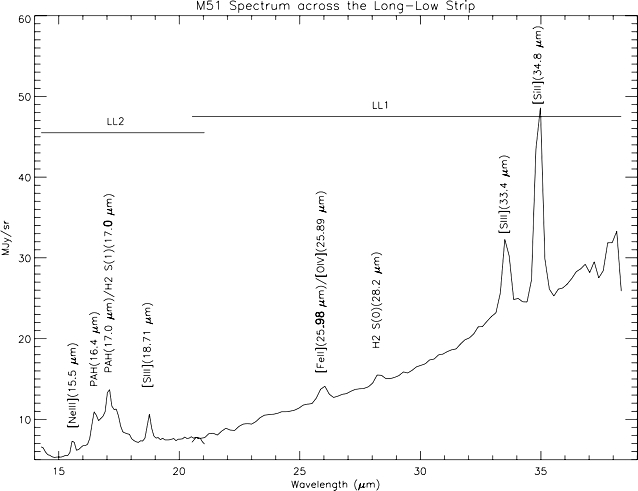
\includegraphics[width=8cm, angle=0]{ll_spec_prop.jpg}
%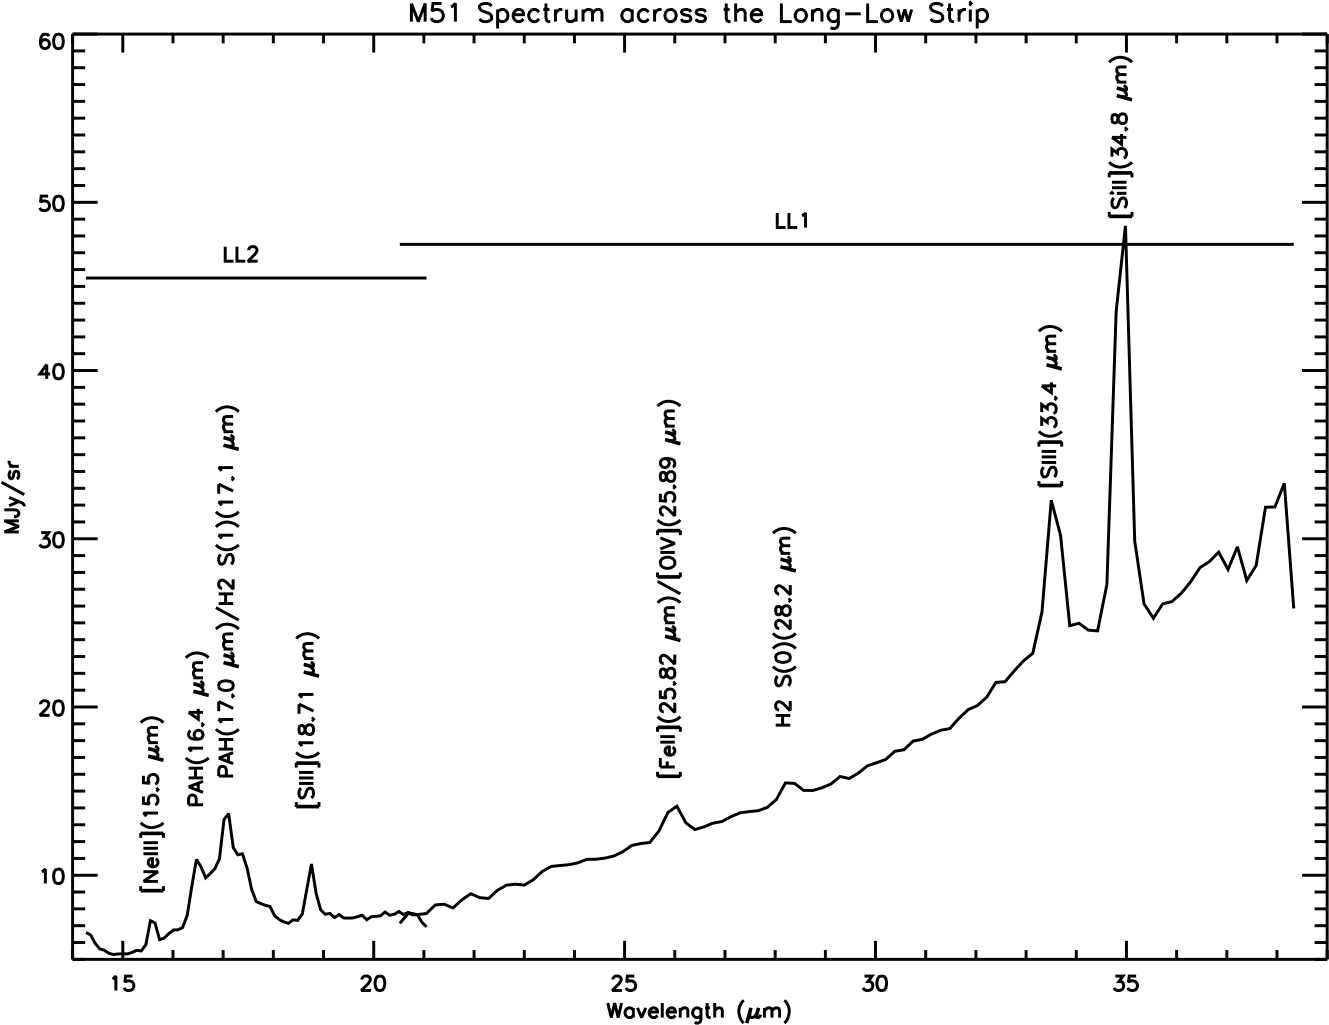
\includegraphics[width=8cm, angle=0]{good_LL_spectrum.jpg}
\hspace{0.1in}
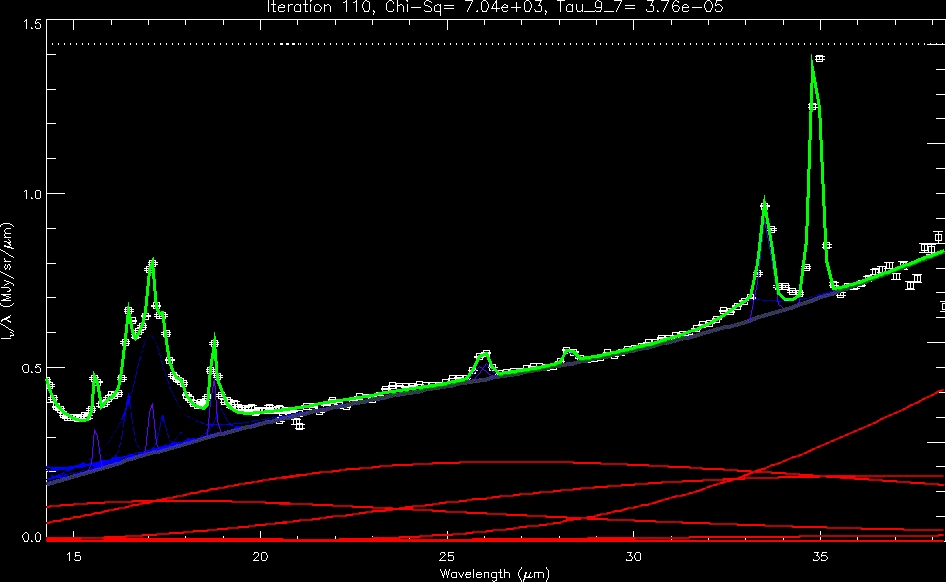
\includegraphics[width=10cm, angle=0]{pahfit.jpg}}}
\caption{{\small $Left$: A sample LL spectrum taken from the M51 strip (GO - 20138) with spectral features noted.  Our study will focus on the $\mathrm{H_2}$ emission across 18 SINGS LL strips. $Right$: We have developed software that processes IRS data cubes and then runs PAHFIT across individual spectra within the data cubes.  In doing so, we create maps of all spectral feature between 14 and 38 $\mu$m.  Here we display a sample PAHFIT spectrum from M51.  The green line is the fit to the entire spectrum, the grey line is the fit to the continuum, the blue gaussian-lorentzians are measurements of PAH features, and the purple lines are the gaussian-lorentzian fits to individual spectral lines.}
\label{figure2}}
%\end{figure}

%\begin{table}
%\begin{center}
%\caption{Galaxies for which there are both SINGS and SONG data available.\label{tbl-1}}
%\begin{tabular}{|rrr|}
%\hline
%NGC 0628 & NGC 3347 & NGC 1111\\
%NGC 1111 & NGC 2780 & NGC 1111\\
%NGC 1111 & NGC 2921 & NGC 1111\\
%NGC 1111 & NGC 3273 & NGC 1111\\
%NGC 1111 & NGC 9607 & $\mathrm{^*}$NGC 1234\\
%NGC 1111 & NGC 3163 & $\mathrm{^*}$NGC 1234\\
%\hline
%\end{tabular}
%\caption{{\small Galaxies for which there are both SINGS and SONG data available.  The $\mathrm{^*}$ %denotes a galaxy for which the SINGS LL  data cubes will be available in SINGS data releave 5 (DR 5).  %SINGS LL data cubes are curently available for all other galaxies.}\label{tbl-1}}
%\end{center}
%\end{table}
%{\bf Figure 1}: SINGS IRS spectral mapping footprints for NGC 2403.  The long strip red and yellow strips across the galaxies are the LL1 and LL2 coverage respectively.  The three rectangles across the central region of the galaxy are the SL1 and SL2 observations.  The two smaller sets of footprints over the nucleus are the Spitzer IRS short-high (SH) and long-high (LH) observatios.  SINGS has acquired similar data sets for 65 galaxies, 18 of which have been observed by BIMA SONG.  SINGS has only studied $\mathrm{H_2}$ for the nuclear regions of each galaxy where the short high (SH), long-high (LH), long-low (LL) observations overlap.  SINGS has not taken advantage of the spectacular IRS LL coverage across the disks of galaxies.  The blue and red boxes in the bottom right of the image are IRS peak up observations.




\centering
%\centerline{\hbox{\hspace{0.0in}
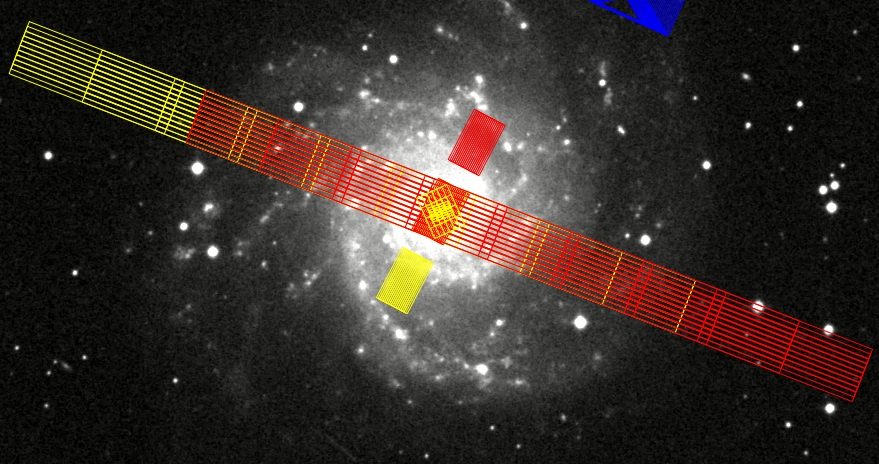
\includegraphics[width=10cm, angle=0]{ngc0628.jpg}
\hspace{0.1in}
\caption{{\small SINGS IRS spectral mapping footprints for NGC 0628.  The long red and yellow strips across the galaxy are the LL1 and LL2 coverage respectively.  The three smaller parallel rectangles across the central region of the galaxy are the SL1 and SL2 observations.  The two smaller sets of footprints over the nucleus are the Spitzer IRS short-high (SH) and long-high (LH) observations.  SINGS has acquired similar data sets for 65 galaxies, 18 have been observed by BIMA SONG.  
%SINGS has only studied $\mathrm{H_2}$ for the nuclear regions of each galaxy where the short high (SH), short-low (SL), long-high (LH),� and long-low (LL) observations overlap.  SINGS has not taken advantage of the spectacular IRS LL coverage across the disks of galaxies.  
}\label{figure2}}


%(b.) We have developed a pipeline that runs PAHFIT across individual spectra in IRS spectral mapping data cubes.  Here we show an example of running PAHFIT on a single spectrum (right).  The green line is the fit to the entire spectrum, the grey line is the fit to the continuum, the blue gaussian-lorentzians are measurements of PAH features, and the purple lines are the gaussian-lorentzian fits to individual spectral lines.}\label{figure2}}
\end{figure}

\clearpage

%We have developed a pipelines that runs PAHFIT across individual spectra in IRS spectral mapping data cubes.  Here we display a sample PAHFIT spectrum from M51.  The green line is the fit to the entire spectrum, the grey line is the fit to the continuum, the blue gaussian-lorentzians are measurements of PAH features, and the purple lines are the gaussian-lorentzian fits to individual spectral lines.
%\label{figure3}}
%\end{figure}

\begin{figure}
\subfigure
\centering
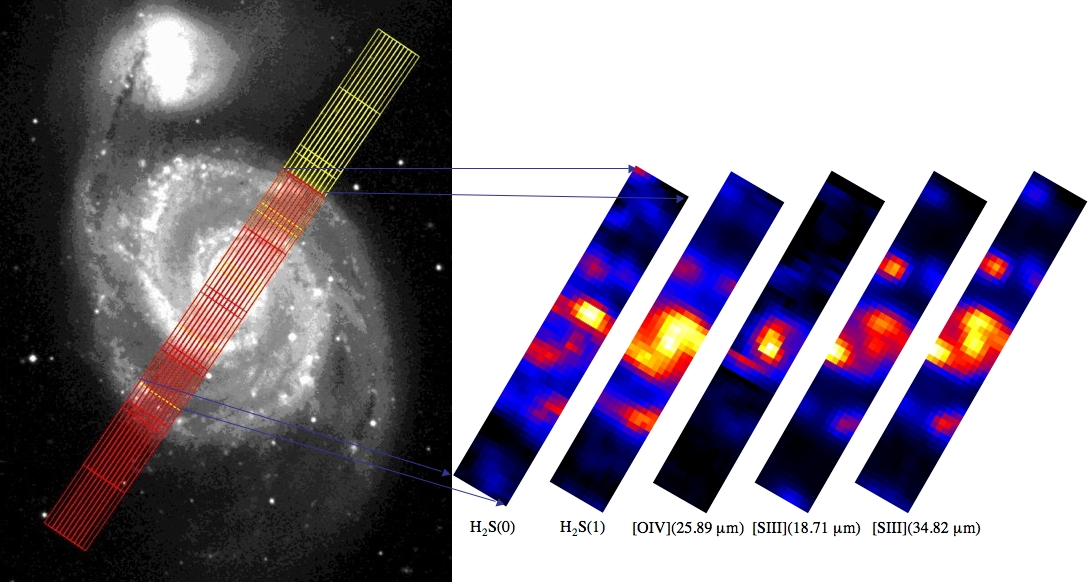
\includegraphics[width=17.5cm, angle=0]{m51maps.jpg}
\hspace{0.5in}
\caption{{\small Shown are the IRS LL spectral mapping AORs ($left$) and maps of the $\mathrm{H_2}$ S(0) (28.2 $\mu$m), $\mathrm{H_2}$ S(1) (17.0 $\mu$m), [OIV](25.89 $\mu$m), [SIII](18.71 $\mu$m), and [SIII](33.82 $\mu$m) lines ($right$) for M51a (GO - 20138).  Maps of the individual lines were created with our software.  The resolution of each map is 5.08 arcsec/pixel. For M51a, this corresponds to about 55 $\mathrm{kpc^2}$ within our beam.}\label{figure3}}\\

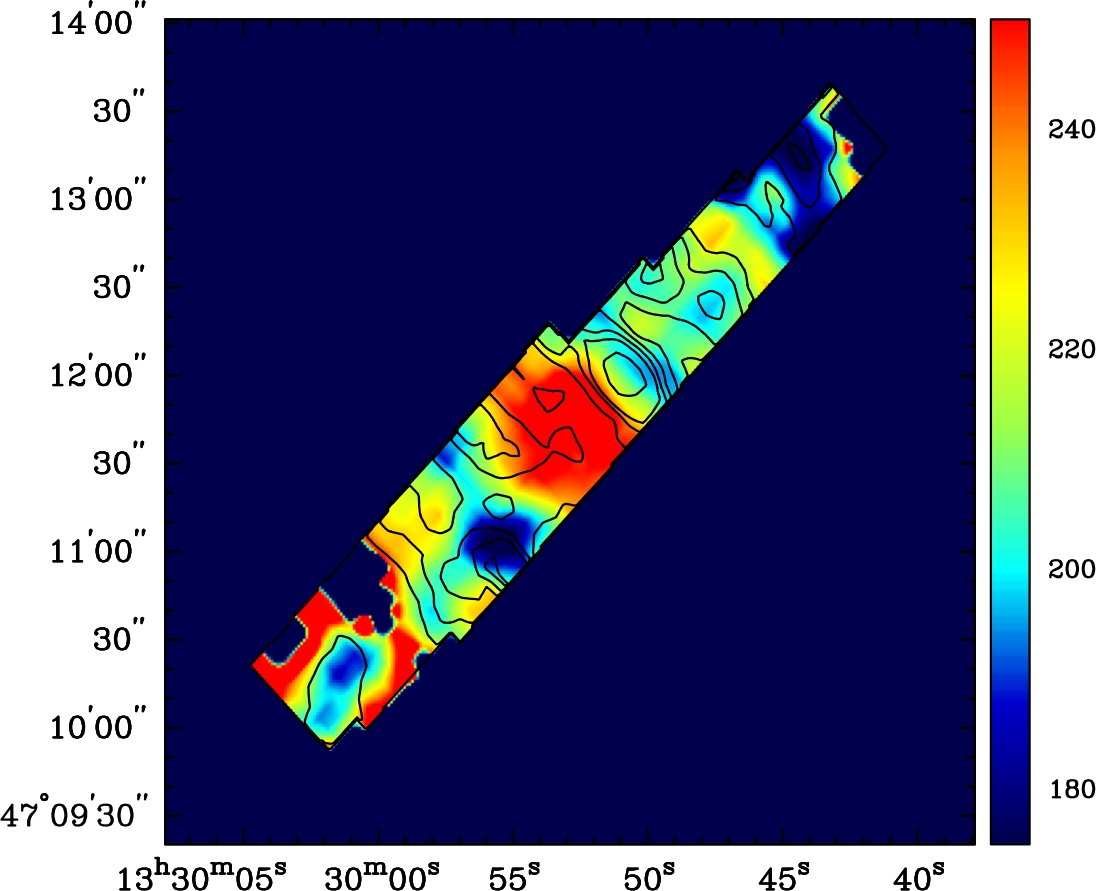
\includegraphics[width=9cm, angle=0]{color_temp_mass_cold.jpg}
\hspace{0.1in}
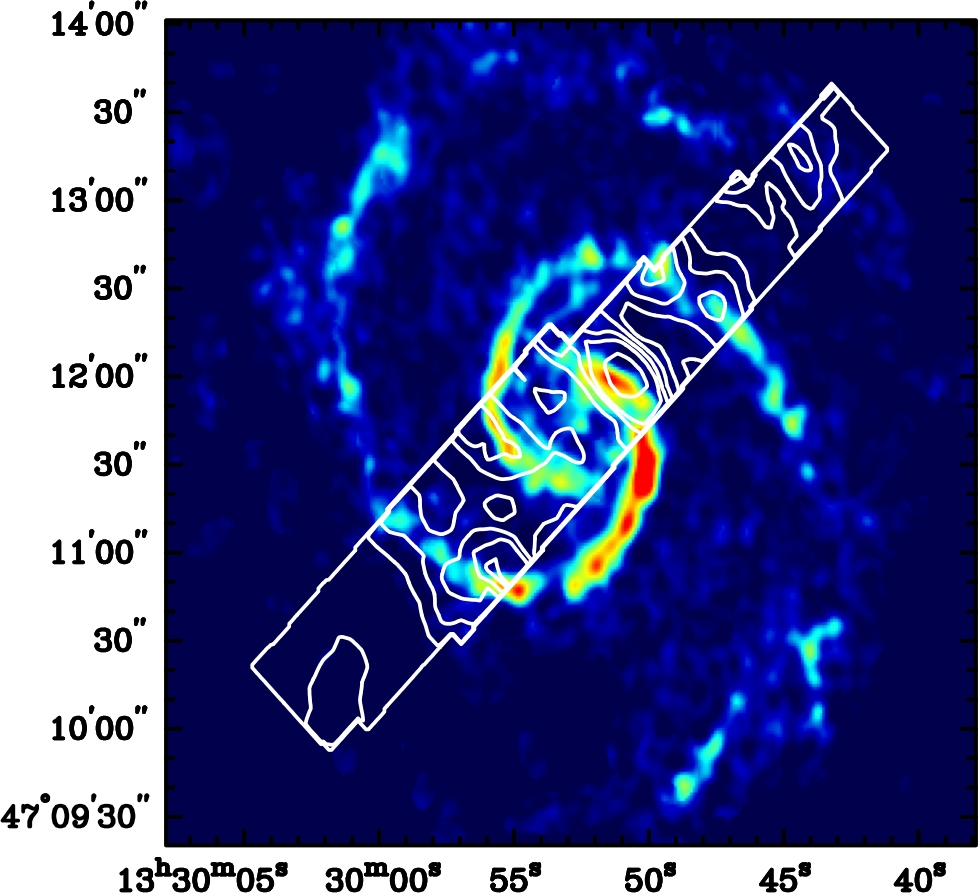
\includegraphics[width=8cm, angle=0]{proposal_co_v_h2.jpg}}}
\caption{{\small $Left$: Map of the warm (T = 100 - 300) $\mathrm{H_2}$ mass distribution (in contours) plotted over the excitation-temperature distribution (in color).  The excitation-temperature is in units of Kelvin; the contours are spaced at 0.5, 0.3, 0.25, 0.20, 0.12, and 0.06 $\mathrm{M_{sun}}$/$\mathrm{pc^2}$.  $Right$: Comparison of the warm $\mathrm{H_2}$ mass to the cold (T = 5 - 10 K) $\mathrm{H_2}$ that is traced by CO (J = 1 - 0) emission. The contours are the same as in the plot on the $left$.  The CO map of M51 was obtained by BIMA SONG.  Note the offset of the warm $\mathrm{H_2}$ mass contours from the CO emission in the spiral arms.}\label{figure4}}



\end{figure}


\clearpage

\section{References}
\\
Brunner, G., Sheth, K., Armus, L., Helou, G., Schinnerer, E., Vogel, S., and Wolfire, M., 2007, submitted\\

Calzetti, D. et al. 2005, ApJ, 633, 871\\

Dale, D. et al., 2006, ApJ, 646, 16\\

Helfer, T.T. et al.,  2003, ApJS, 145, 259\\

Higdon, S.J.U., Armus, L., Higdon, J.L., Soifer, B.T., and Spoon, H.W.W., 2006, ApJ, 648, 323\\

Jensen, E.B., Talbot, R.J., and Dufour, R.J., 1981, ApJ, 243, 716\\

Kaufman, M.J., Wolfire, M.G., and Hollenbach, D.J., 2006, ApJ, 644, 283\\

Kennicutt, R.C. et al., 2003, PASP, 115, 928\\

Lutz, D., Kunze, D., Spoon, H.W.W., and Thornley, M.D., 1998, A\&A, 333, L75\\

Regan, M.W. et al., 2001, ApJ, 561, 218\\

Rigopoulou, D., Kunze, D., Lutz, D., Genzel, R., and Moorwood, A.F.M., 2002, A\&A, 389, 374\\

Roussel, H. et al., 2007, in press\\

Sheth, K., Regan, M.W., Vogel, S.N., and Teuben, P.J., 2000, ApJ, 532, 221 \\

Smith, J.D. et al., 2004, ApJS, 154, 199\\

Smith, J.D. et al., 2007, ApJ, 656, 770\\

Schaerer, D. and Stasinska, G., 1999, A\&A, 345, L17\\

Talbot, R.J., Jensen, E.B., and Dufour, R.J., 1979, ApJ, 229, 91\\

Vogel, S.N., Kulkarni, S.R., and Scoville, N.Z., 1988, $Nature$, 334, 402\\

Young, J.S. and Devereux, N.A., 1991, ApJ, 373, 414\\

\clearpage

\section{Brief Resume/Bibliography}

{\bf Student PI}:  Gregory Brunner is a graduate student at Rice University  and a 2006-2007 Spitzer Visiting Graduate Student Fellow.  During the fellowship he worked with Kartik Sheth on IRS spectral mapping data of M51a.  He has developed software that takes IRS low resolution data cubes and creates line flux maps of every spectral feature in the data cube.  He has submitted a draft of the results of a study of the $\mathrm{H_2}$ emission, excitation, and mass across M51a that he completed during the Spitzer Visiting Graduate Student Fellowship.  His thesis will combine the research proposed here with his ongoing research at SSC to study the spatial distribution of $\mathrm{H_2}$ in nearby galaxies.\\

{\bf Administrative PI}: Reginald Dufour is a professor in the Department of Physics and Astronomy at Rice University.  His interests are observational astrophysics of star forming galaxies, HII regions, and shell nebulae.\\

{\bf Co-I}: Kartik Sheth is a research scientist at Spitzer Science Center and a member of the Spitzer IRS instrument team.\\

{\bf Co-I}: Stuart Vogel is a professor of astronomy and the director of the lab for millimeter-wave astronomy at the University of Maryland.  His main research interests are star formation and galaxy evolution.\\

{\bf Co-I}: Mark Wolfire is a research scientist at the University of Maryland.  He is an expert on modeling photo-dissociation regions.\\
\\
{\bf Selected references relevant to this proposal from the team:}\\
\\
 Brunner, G., Sheth, K., Armus, L., Helou, G., Schinnerer, E., Vogel, S., and Wolfire, M., 2007, submitted\\
 
 Dufour, R.J., Talbot, R.J., Jensen, E.B., and Shields, G.A., 1980, ApJ, 236, 119\\
 
 Rubin, R.H., Dufour, R.J., Colgan, R.J., Liao, S.W., Harrington, J.P, Levine, D.A., and Lord, S.D., 2002, RMxAC, 12, 106\\
 
 Moore, B.D., Hester, J.J., and Dufour, R.J., 2004, AJ, 127, 3484\\
 
 Buckalew, B.A., Kobulnicky, H.A., and Dufour, R.J., 2005, ApJSS, 157, 30\\
 
 Sheth, K., Regan, M.W., Vogel, S.N., and Teuben, P.J., 2000, ApJ, 532, 221\\
 
 Sheth, K., Vogel, S.N., Regan, M.W., Teuben, P.J., Harris, A.I. and Thornley, M.D., 2002, AJ, 124, 2581\\
 
 Sheth, K., Blain, A.W., Kneib, J-P., Frayer, D.T., van der Werf, P.P., and Knudsen, K.K., 2004, ApJL, 614, 5\\
 
 Vogel, S.N., Rand, R.J., Gruendl, R.A., and Teuben, P.J., 1993, PASP, 105, 666\\
 
 Vogel, S.N., Kulkarni, S.R., and Scoville, N.Z., 1988, $Nature$, 334, 402\\
 
 Wolfire, M.G., McKee, C.F., Hollenbach, D., and Tielens, A.G.G.M., 2003, ApJ, 586, 278\\
 
 Wolfire, M.G., Hollenbach, D., McKee, C.F., Tielens, A.G.G.M., and Bakes, E.L.O., 1995, ApJ, 443, 152\\

\section{Status of Existing Spitzer Programs}

{\bf Administrative PI} R. Dufour is a Co-I on GO - 3412, GO - 20049, and GO - 20057.  The GO - 3412 IRS observations of HII regions in M83 have been analyzed and submitted for publication to MNRAS.  The GO - 20049 IRS observations of HII regions in M33 have been completed and preliminary results have been presented at AIU symposium number 235 in Prague.  The GO - 20057 IRS observations of three halo PNe are pending completion and analysis of the data is ongoing.\\

{\bf Co-I} K.\ Sheth is the PI for GO - 20138.
% and Co-I on GO - 20587.  The
GO - 20138 IRS observations of M51a have been reduced and analyzed and the results for $\mathrm{H_2}$ in M51a have been submitted.\\  
%The GO - 20587 IRS observations have been reduced and are currently under analysis.\\

%{\bf Co-I} S.\ Vogel is a Co-I on GO - 20138 and GO - 20587. \\

{\bf Co-I} M. Wolfire is PI on GO - 3679, GO 20012, GO- 20097, and GO - 30295.  For GO - 3679, GO - 20012, and GO - 20097 all of the data has been taken and are currently under analysis.  Results from of the analysis of PDRs from GO - 3679 presented in Povich et al., 2007, ApJ.  Results for the analysis of data from of GO - 3679 and GO - 20097 on $\mathrm{H_2}$ in PDRs is in preparation.\\

\section{Financial Contact Information}

For PIs G. Brunner and R. Dufour\\
Dr. Heidi L. Thornton\\
heidi@rice.edu\\
Assistant Director of Sponsored Research\\
Office of Sponsored Research MS-16\\
Rice University\\
Houston, TX 77005-1892\\
713-348-6204 \\
\\
For Co-I K. Sheth\\
Eloise Kennedy\\
eks@ipac.caltech.edu\\
Image Processing and Analysis Center\\
MS-220-6\\
Pasadena, CA 91125\\
626.395.1801\\
\\
%For Co-Is S. Vogel and M. Wolfire\\
%Monique Anderson, Contract Manager\\
%manderson@umresearch.umd.edu\\
%University of Maryland, College Park\\
%3112 Lee Building\\
%College Park, MD 20742\\
%301.405.6272\\

\section{Cost Plan and Budget Narrative}

Below is the narrative for the Rice University Cost Plan (R. J. Dufour, administrative PI) for which the proposal PI, Greg Brunner, is a graduate student.  The total of the Rice cost plan for the 1 year period beginning 1 October 2007 is \$81,765.  Separately Dr. Kartik Sheth of the Spitzer Science Center is requesting \$15,000 support during this period though SSC.  CoIs  Vogel and Wolfire of the University of Maryland are not requesting separate support.  Therefore, the total support requested for this archival project is \$96,765.\\

The primary direct cost items are salaries for G. Brunner and R. Dufour.  Since the scientific PI will be a third-year graduate student in October 2007, the stipend will be \$24,700 per year (assuming he will qualify for Ph. D. candidacy in September 2007).  Brunner just completed six months of residency at SSC as a Graduate Student Fellow working with Sheth et al. on $\mathrm{H_2}$ mapping of M51.  Currently this is being submitted for publication and also will be submitted and defended by Brunner for Ph.D. candidacy during the summer of 2007.  If this proposal is approved, then the described research will be a major part of Brunner�s Ph.D. dissertation.  As noted in the proposal, Brunner will be analyzing 2D IRS observations and mapping of molecular hydrogen properties across 18 galaxies previously observed by SINGS, which is a massive amount of data reduction, including comparison with IR-visible imagery of the galaxies.  Realistically, such a large project will take longer than a year, but here we are limited to proposing for the first year of research (given some will have already been done by the time the funding is in place).  Currently Brunner is being supported by AURA/HST grants involving UV-optical imagery/spectroscopy of emission nebulae and can only work part time on the Spitzer $\mathrm{H_2}$ mapping.  However, this should be nearly completed in late 2007 so he will be able to pursue this proposed research full time when funding is in place.\\

R. Dufour is a Professor of Physics and Astronomy at Rice University and has been at Rice since 1976 studying star-forming galaxies and nebulae.  He will be Brunner�s primary thesis advisor and administrative PI for this project.  He is requesting one month of summer salary support (\$10,395).  Dufour expects to become involved in the project scientifically as well as administratively at a level of approximately 3 weeks per semester (Rice permits up to 50\% of the academic time for research during the 9-month school year) and 1 month during the summer.\\

Other direct cost items include \$4,200 in travel for Brunner to take ~5-day trips to SSC to consult with Sheth, to the University of Maryland to consult with Vogel and Wolfire, and one domestic scientific meeting (e.g. AAS) to present the results of this research.  Additionally, \$4,200 is requested for publication costs (approximately two ~15 page ApJ or AJ articles) -which is arguably conservative given the large amount of data and galaxies proposed to be studied.  Modest amounts is requested for research materials and supplies (\$600) and computer services (\$1200 -- IDL, user fees, and maintenance support).  No equipment is requested, all of the hardware (and software) necessary for the project is in place at Rice.\\

Therefore the direct costs are \$35,095 (salaries), \$4,200 (travel), and \$6,000 (publications, maintenance, and supplies) = \$57,332 total.  Fringe benefits on the salaries is \$12,307 and indirect costs are \$24,453.  Therefore, the total is \$81,785 for the Rice University share of the project cost.\\



\clearpage
\begin{table}[ht]
\caption{Spitzer Cycle-4 Budget 1 Oct 2007 -- 30 Sep 2008}
\begin{tabular}{|l|l|l|l|l|}
\hline
Narrative & & & & \\
\hline
Footnote & Cost Element & & & \\
\hline
\hline
 & Direct Labor Hours (by labor category) & Hours & Rate & Amount\\
\hline
 & G. Brunner - Student PI & 12 months & 2058.33/mo & 24,700.00 \\
\hline
 & R. Dufour - Admin. PI & 1 month & 10,395.00/mo & 10,395.00 \\
\hline
 & Fringe benefits (see attachments) & & & 12,037.00 \\
\hline
 & & & & \\
\hline
 & & & & \\
\hline
 & & & & \\
\hline
 & & & & \\
\hline
 & Total Direct Labor & & & 47,132.00 \\
\hline
\hline
 & Overhead & Base & Rate & \\
\hline
 & See attachments & & & 24,453.00 \\
\hline
 & & & & \\
\hline
 & & & & \\
\hline
 & & & & \\
\hline
 & & & & \\
\hline
 & & & & \\
\hline
 & & & & \\
\hline
 & Total Overhead & & & 24,453.00 \\
\hline
\hline
 & Material Costs & & & \\
\hline
 & Material Burden & & & \\
\hline
 & Total Material & & & \\
\hline
\hline
 & Subcontract Cost & & & \\
\hline
 & Subcontract Burden & & & \\
\hline
 & Total Subcontract & & &\\
\hline
\hline
 & Other Direct Cost (ODC) & & & \\
\hline
 & Travel, Publication, Computer Costs & & & 10,200.00 \\
\hline
 & & & & \\
\hline
 & & & & \\
\hline
 & & & & \\
\hline
 & & & & \\
\hline
 & Total ODC & & & 10,200.00 \\
\hline
\hline
 & Sub-Total Cost & & & 81,785.00 \\
\hline
 & Total General \& Administrative & & & \\
\hline
 & Total Cost & & & 81,785.00  \\
\hline
\end{tabular}
\end{table}

\end{document}